\documentclass[a4paper,12pt,reqno]{amsart}
\usepackage{amssymb}
\usepackage{enumerate}
\usepackage{ifthen}
\pagestyle{plain}
\renewcommand{\baselinestretch}{1.4}
\usepackage{tikz}
\usepackage{amsmath}
\usepackage{amssymb}
\usepackage{pgfplots}
\usepackage{pgfplotstable}
\usepgfplotslibrary{fillbetween}
\usepackage{graphicx}
\usepackage[colorlinks=true, allcolors=blue]{hyperref}
\usepackage[english]{babel}
\setlength{\textwidth}{16cm}
\setlength{\textheight}{24cm}
\setlength{\oddsidemargin}{0cm}
\setlength{\topmargin}{-0.5cm}
\setlength{\evensidemargin}{0cm}
\setlength{\footskip}{40pt}
\setlength{\arrayrulewidth}{0.5mm}
\setlength{\tabcolsep}{18pt}
\renewcommand{\arraystretch}{1.5}
\pgfplotsset{width = 10cm,compat=newest}

\title{Linear Regression , Logistic Regression and Gaussian Discriminant Analysis}
\author{Ashish Kumar}

\begin{document}

\maketitle
\begin{gather*}
    \address{Department Of Mathematics, IIT Roorkee, Roorkee - 247667}\\
\email{a\_kumar1@ma.iitr.ac.in}
\end{gather*}

\keywords{Linear Regression, Logistic Regression, Multivariate Normal Distribution, Gaussian Discriminant Analysis Model}\\

\begin{abstract}
    The article provides an overview of several fundamental statistical modeling techniques, including linear regression, logistic regression, multivariate normal distribution, and Gaussian discriminant analysis model. It explains how these techniques are used to analyze relationships between variables and make predictions based on data. The article covers the underlying assumptions, methods, and applications of each technique, providing readers with a clear understanding of their strengths and limitations. Whether you are a novice or an experienced data analyst, this article should act as an introduction for gaining a deeper understanding of these essential statistical techniques.
\end{abstract}
\renewcommand{\thefootnote}{\fnsymbol{footnote}}
\footnote[0]{\textit{AMS classification:} 62J05,62J12,62H10,62H30}
\pagebreak
\tableofcontents
\pagebreak
\section{Linear Regression}
\subsection{Introduction}
Linear Regression is a statistical supervised learning technique to predict the quantitative variable by forming a linear relationship with one or more independent features.\\
The goal of linear regression is to find the line of best fit that describes the relationship between the two variables. The line of best fit is a straight line that minimizes the distance between the predicted values and the actual values. 

\begin{center}
\begin{tikzpicture}
\begin{axis}[    xlabel=$x$,    ylabel=$y$,    xmin=0,xmax=10,    ymin=0,ymax=20,    axis lines=middle,    xtick={0,2,...,10},    ytick={0,5,...,20},    ]
    \addplot[only marks,color=blue,mark=*] coordinates {
    (1,3.5)
    (2,4)
    (3,8)
    (4,9)
    (5,11)
    };
    \addplot[color=red,domain=0:10]{2*x+1};
    \legend{Data,Regression Line}
\end{axis}
\end{tikzpicture}\\
An example of Linear Regression
\end{center}

\subsection{Line of best fit}
To relate independent variable with a dependent variable , the simplest linear function we can think of would be 

\begin{equation} \label{eq1}
h_{\theta}(x) = \theta_0 + \theta_{1}x_{1} + \theta_{2}x_{2} ...
\end{equation}

where $\theta_{i}$'s are called weights. Here $\theta_0$ would be the intercept term. Hence
\begin{equation} \label{eq2}
h(x) = \sum_{i=0}^{n} \theta_{i}x_{i} = \theta^{T}x,
\end{equation} 
where $\theta =  
\begin{bmatrix}
\theta_0 \\
\theta_1 \\
\theta_2 \\
\vdots
\end{bmatrix}
$
and 
$
X = 
\begin{bmatrix}
1 \\
x_1 \\
x_2 \\
\vdots
\end{bmatrix}
$
\subsection{Cost Function}
We define cost function as 
\begin{equation} \label{eq3}
J(\theta) = \frac{1}{2}\sum_{i=1}^{n}(h_{\theta}(x^{(i)}) - y^{(i)})
\end{equation}
which is basically how far the $h(x^{(i)})$'s are from the $y^{(i)}$'s.
For our line \ref{eq1} to be the best line , the cost function should be the minimum.
\subsection{LMS}
We need to minimize $J(\theta)$. We can do that by the $\textbf{gradient descent algorithms}$.We will not go deep into the algorithm due to the scope of this article.Applying it to the given sample for minimizing the cost function yields,
\begin{equation} \label{eq4}
\theta_{j} := \theta_{j} + \alpha(y^{(i)}-h_{\theta}(x^{(i)}))x_j^{(i)}
\end{equation}
This is called as $\textbf{LMS}$ update rule or $\textbf{Widrow-Hoff}$ learning rule.By grouping the updates of the coordinates into an update of the vector $\theta$, we can write the same equation better as 
\begin{equation} \label{eq5}
\theta := \theta + \alpha \sum_{i=1}^{n}(y^{(i)} - h_{\theta}(x^{(i)}))x^{(i)}
\end{equation}
This method looks at every example in the entire training set on every step, and is called $\textbf{batch gradient descent}$.
\subsection{Shortcomings of Linear Regression}
The shortcomings are the assumptions we take: 
\begin{enumerate}
    \item Linearity Assumption: Linear regression assumes that the relationship between the dependent variable
    \item Outliers: Linear regression is sensitive to outliers in the data.
    \item Over-fitting: Linear regression can be prone to over-fitting, especially when there are many independent variables. 
    \item Causality: Linear regression only captures the correlation between the dependent variable and independent variables.
\end{enumerate}
\section{Learning Algorithms}

\subsection{Discriminative Learning Algorithms : }
Consider a given set of data points and you need to classify them based on certain features. Classic algorithms like logistic regression or perceptron algorithm classifies the given set by fitting a straight line (or a decision boundary) in the data model. Then it classifies a new entry based on which part it fell.
These "direct" algorithms which maps space of inputs $\textbf{X}$ to the set $\{0,1\}$ are called $\textbf{discriminative learning algorithms}$.

\subsection{Generative Learning Algorithms : }
Alternate to the previous approach, we can instead create a model based on the given features and then given a new entry, goes ahead to compare it to both models to find the likeliness and decide based on this info.\\
Now consider the algorithms that instead try to model $p(x|y)$.These algorithms are known as $\textbf{generative learning algorithms}$.\\
How does this work ? 
After modelling the $\textbf{class priors}$ i.e, $p(y)$ and $p(x|y)$, now given a new entry (i.e, x) we need to find $p(y|x)$ which can be found using the Bayes rule :
$$p(y|x) = \frac{p(x|y)p(y)}{p(x)}$$ or
\begin{equation} \label{eq6}
p(y|x) = \frac{p(x|y)p(y)}{p(x|y = 1)p(y = 1) + p(x|y = 0)p(y = 0)}
\end{equation}

% --------------------(Clarity)-----------------------------

\section{Multivariate Normal Distribution}
\begin{flushleft}
Also known as Multivariate Gaussian Distribution (${N(\mu,\Sigma)}$), the Multivariate Normal Distribution in $d$-dimensions is given by :

\begin{equation} \label{eq7}
p(x;\mu,\Sigma) = {\frac{1}{(2\pi)^{d/2}|\Sigma|^{1/2}} \exp\left(-\frac{1}{2}(x-\mu)^T \Sigma^{-1} (x-\mu)\right)}
\end{equation}
 where $|\Sigma|$ denotes the determinant of the covariance matrix,which is symmetrical and positive semi-definite and the \textbf{mean vector}$\, \mu \in \mathbb{R}^d$ and \textbf{covariance matrix}$\, \Sigma \in \mathbb{R}^{dxd}$.
 
If a random variable X is a vector , then it's mean is given by $\mu$ : 
\begin{equation} \label{eq8}
E(X) = \int_{x} x p(x;\mu,\Sigma) dx = \mu
\end{equation} 
and the covariance is given by :
\begin{equation} \label{eq9}
Cov(Z) = E[(Z-E[Z])(Z-E[Z])^T]
\end{equation} 
Here is an example of what the density of a Gaussain distribution looks like :\newline

\begin{center}
\def\centerx{0}
\def\centery{0}

\begin{tikzpicture}
\begin{axis}
\addplot3[surf,domain=-3:3,domain y=-5:5] 
        {exp(-( (x-\centerx)^2 + (y-\centery)^2)/2 )};
    \node[circle,inner sep=1pt,fill=blue,pin=90:$\mu$] 
        at (axis cs:\centerx,\centery,1) {};
\end{axis}
\end{tikzpicture}\\
An example of a normal distribution with $\mu = 
\begin{bmatrix}
0  \\
0 
\end{bmatrix}
 and \; \Sigma =  
\begin{bmatrix}
1 & 0 \\
0 & 1
\end{bmatrix}
$
\end{center}
\end{flushleft}

% --------------------(Clarity)-----------------------------

\section{Gaussian discriminant analysis model}


A generative learning algorithm where $p(x|y)$ is distributed according to a multivariate normal distribution is Gaussian discriminant analysis (GDA).

Given input features x as continuous random variables,GDA models $p(x|y)$ using the above multivariate normal distribution.

$$ y \sim Bernoulli(\phi) \; or \; p(y) = {\phi}^y{1-\phi}^{1-y}$$
$$x|y = 0 \sim N({\mu}_0,\Sigma)$$
$$x|y = 1 \sim N({\mu}_1,\Sigma)$$
Finding the log-likelihood of the data :
$$ 
l(\phi, \mu_0, \mu_1, \Sigma) = \log {\Pi_{i=1}^n} \, Y p(x^{(i)}, y^{(i)}; \phi, \mu_0, \mu_1, \Sigma)
$$
$$
\qquad \; = \log {\Pi_{i=1}^n} \, Y p(x^{(i)}|y^{(i)}; \mu_0, \mu_1, \Sigma)p(y^{(i)}; \phi)
$$\newline
By maximizing $l$ with respect to the parameters, we will find the maximum likelihood estimate of the parameters to be :

\begin{equation} \label{eq10}
\phi = \frac{1}{n} \sum_{i=1}^{n} 1\{{y^{(i)}=1}\}
\end{equation} 
\begin{equation} \label{eq11}
\mu_0 = \frac{\sum_{i=1}^{n} 1\{y^{(i)}=0\}x(i)}{\sum_{i=1}^{n} 1\{y^{(i)}=0\}}
\end{equation} 
\begin{equation} \label{eq12}
\mu_1 = \frac{\sum_{i=1}^{n} 1\{y^{(i)}=1\}x(i)}{\sum_{i=1}^{n} 1\{y^{(i)}=1\}}
\end{equation} 
\begin{equation} \label{eq13}
\Sigma = \frac{1}{n} \sum_{i=1}^{n} (x^{(i)} - \mu_{y(i)}) (x^{(i)} - \mu_{y(i)})^T
\end{equation} 
Here is an example of classification done for a data set using GDA.

\begin{center}
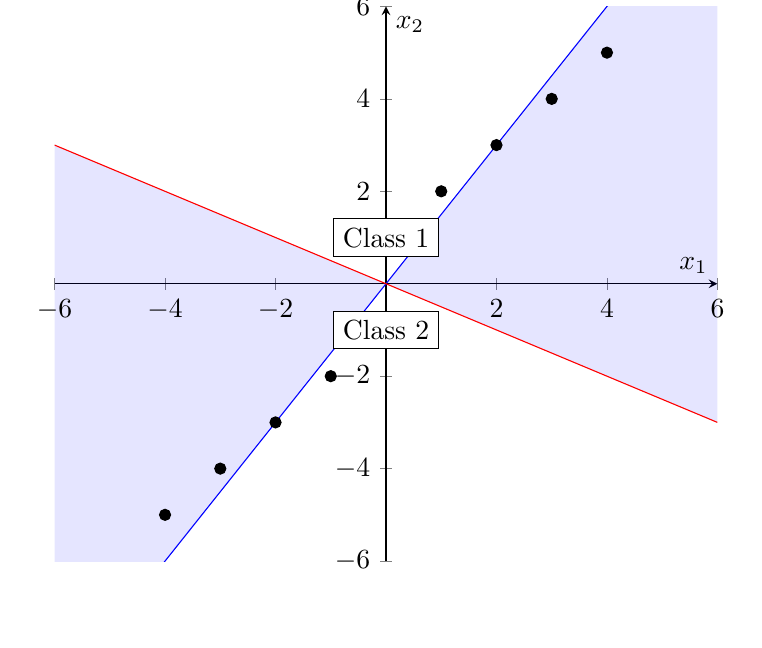
\begin{tikzpicture}
\begin{axis}[
xlabel=$x_1$,    
ylabel=$x_2$,   
xmin=-6,
xmax=6,    
ymin=-6,
ymax=6,    
axis lines=middle,    
xtick={-6,-4,...,6},    
ytick={-6,-4,...,6},    ]
\addplot[name path=A,domain=-6:6,samples=100,color=blue]{1.5*x};
\addplot[name path=B,domain=-6:6,samples=100,color=red]{-0.5*x};
\addplot[fill=blue,opacity=0.1] fill between[of=A and B,soft clip={domain=-6:6}];
\addplot[only marks,mark=*,color=black] coordinates {
(1,2)
(2,3)
(3,4)
(4,5)
(-1,-2)
(-2,-3)
(-3,-4)
(-4,-5)
};
\node[draw,fill=white] at (axis cs: 0,1) {Class 1};
\node[draw,fill=white] at (axis cs: 0,-1) {Class 2};
\end{axis}
\end{tikzpicture}
\end{center}

% --------------------(Clarity)-----------------------------

\section{GDA and logistic regression}
Now that we have understood GDA in brief, we will see how GDA is connected to logistic regression and which is better.
\subsection{Logistic Regression}
Logistic regression is a binary classification strategy. It is closely similar to Linear Regression. The basic idea is to fit a sigmoid function in the model instead of fitting a striaght line.
\subsection{Sigmoid Function}
Logistic or sigmoid function is of form $$g(z) = \frac{1}{1+{e^{-z}}}$$ Upon plotting, it looks like : \newline
\begin{center} 
\begin{tikzpicture}
\begin{axis}[
    axis lines = left,
    xlabel = \(z\),
    ylabel = {\(f(z)\)},
]
\addplot [
    domain=-5:5, 
    samples=100,
    thick, blue] {1/(1+exp(-x)};
    color=red,
]
\end{axis}
\end{tikzpicture}
\end{center}

Also note that, $g'(z) = g(z)(1 - g(z))$

We change out hypothesis such as $$h_{\theta}(x) = g(\theta^{T}x) = \frac{1}{1+{e^{-\theta^{T}x}}}$$.

Given this model, we can write :
$$p(y|x;\theta) = (h_{\theta}(x))^{y}(1 - h_{\theta}(x))^{1 - y}$$

for n training examples , (asssuming they were generated independently) 
$$L(\theta) = p(\overrightarrow{y}| \mathbb{X};\theta) = \Pi_{i=1}^n \, p(y_{(i)}|x_{(i)};\theta)$$
Taking the log and maximizing with respect to the parameters using gradiant descent rule :
\begin{equation} \label{eq14}
\theta_{j} = \theta_{j} + \alpha(y^{(i)} - h_{\theta}(x^{(i)}))x^{(i)}_j
\end{equation}

\subsection{Which is better? :  GDA or Logistic Regression?}

If we view the quantity $p(y = 1|x; \varphi, \mu_0, \mu_1, \Sigma)$ as a function of $x$, we'll find that it can be expressed in the form
$$
p(y = 1|x; \phi, \Sigma, \mu_0, \mu_1) = \frac{1}{1 + e^{-\theta^T x}}
$$ which is very similar to the logistic regression form. So, which is better ? Let us compare them in a table. \newline \newline
\begin{tabular}{ |p{6cm}|p{6cm}|  }
\hline
\multicolumn{2}{|c|}{Differences b/w GDA and Logistic Regression} \\
\hline
Logistic Regression & GDA \\
\hline
Used for binary classification problems  & Optimization algorithm used to minimize the cost function  \\
Logistic regression updates the model parameters based on the training data, by minimizing the error between the predicted output and the actual output.   & Gradient descent, on the other hand, updates the model parameters by minimizing the cost function, which is a measure of the error between the predicted output and the actual output. \\
Takes long time to converge to local minima & Faster to converge than LR \\
Good choice when you have a binary classification problem & Good choice when you need to optimize the parameters of a cost function \\
\hline
\end{tabular}\newline\newline
Basically GDA makes stronger modeling assumptions about the data than does logistic regression. When these assumptions are correct, GDA forms a better model but if you are uncertain about the assumptions, esp. in large datasets, it would be better to use logistic regression to classify.

\bibliographystyle{alpha}
\bibliography{sample}

\end{document}
